\documentclass[tikz,border=8pt]{standalone}
% Shared look for every TikZ diagram. Load with % Shared look for every TikZ diagram. Load with % Shared look for every TikZ diagram. Load with \input{../../tools/tikz-style.tex}
\usepackage[T1]{fontenc}
\usepackage{lmodern}
\renewcommand{\sfdefault}{lmr}  % diagrams use the same serif as the text
\usetikzlibrary{arrows.meta, positioning, shapes.geometric, calc, fit, backgrounds}
\definecolor{cblue}{HTML}{4C78A8}
\definecolor{corange}{HTML}{F58518}
\definecolor{cgreen}{HTML}{54A24B}
\definecolor{cred}{HTML}{E45756}
\definecolor{cpurple}{HTML}{B279A2}
\definecolor{cgrey}{HTML}{6B6B6B}
\tikzset{
  every picture/.style={font=\sffamily, line width=1.2pt},
  box/.style={draw=#1, fill=#1!12, rounded corners=4pt, align=center, inner sep=7pt, minimum height=1.1cm},
  box/.default=cgrey,
  arrow/.style={-{Stealth[length=3mm]}, draw=cgrey, line width=1.4pt},
  title/.style={font=\sffamily\bfseries\Large},
  note/.style={font=\sffamily\small, text=cgrey, align=center},
}
\AtBeginDocument{\hyphenpenalty=10000 \exhyphenpenalty=10000}

\usepackage[T1]{fontenc}
\usepackage{lmodern}
\renewcommand{\sfdefault}{lmr}  % diagrams use the same serif as the text
\usetikzlibrary{arrows.meta, positioning, shapes.geometric, calc, fit, backgrounds}
\definecolor{cblue}{HTML}{4C78A8}
\definecolor{corange}{HTML}{F58518}
\definecolor{cgreen}{HTML}{54A24B}
\definecolor{cred}{HTML}{E45756}
\definecolor{cpurple}{HTML}{B279A2}
\definecolor{cgrey}{HTML}{6B6B6B}
\tikzset{
  every picture/.style={font=\sffamily, line width=1.2pt},
  box/.style={draw=#1, fill=#1!12, rounded corners=4pt, align=center, inner sep=7pt, minimum height=1.1cm},
  box/.default=cgrey,
  arrow/.style={-{Stealth[length=3mm]}, draw=cgrey, line width=1.4pt},
  title/.style={font=\sffamily\bfseries\Large},
  note/.style={font=\sffamily\small, text=cgrey, align=center},
}
\AtBeginDocument{\hyphenpenalty=10000 \exhyphenpenalty=10000}

\usepackage[T1]{fontenc}
\usepackage{lmodern}
\renewcommand{\sfdefault}{lmr}  % diagrams use the same serif as the text
\usetikzlibrary{arrows.meta, positioning, shapes.geometric, calc, fit, backgrounds}
\definecolor{cblue}{HTML}{4C78A8}
\definecolor{corange}{HTML}{F58518}
\definecolor{cgreen}{HTML}{54A24B}
\definecolor{cred}{HTML}{E45756}
\definecolor{cpurple}{HTML}{B279A2}
\definecolor{cgrey}{HTML}{6B6B6B}
\tikzset{
  every picture/.style={font=\sffamily, line width=1.2pt},
  box/.style={draw=#1, fill=#1!12, rounded corners=4pt, align=center, inner sep=7pt, minimum height=1.1cm},
  box/.default=cgrey,
  arrow/.style={-{Stealth[length=3mm]}, draw=cgrey, line width=1.4pt},
  title/.style={font=\sffamily\bfseries\Large},
  note/.style={font=\sffamily\small, text=cgrey, align=center},
}
\AtBeginDocument{\hyphenpenalty=10000 \exhyphenpenalty=10000}

\usetikzlibrary{matrix}
% Decoding a formula: shrink to 2 points and 2 components, then write out every case.
\begin{document}
\begin{tikzpicture}[every node/.append style={font=\large}]
  \node[box=cgrey, text width=7.6cm] (f) at (0,0) {$\displaystyle \gamma_k(x_i) = \frac{\pi_k\, p(x_i \mid k)}{\sum_{j=1}^{K} \pi_j\, p(x_i \mid j)}$\\[6pt] for each point $x_i$ and each component $k$};
  \node[box=corange, text width=5.6cm, right=1.6cm of f] (s) {shrink to 2 cases:\\ points $x_1, x_2$\\ components $k = 1, 2$, so $K = 2$};
  \draw[arrow] (f) -- (s);
  \matrix[below=1.4cm of $(f.south)!0.5!(s.south)$, matrix of nodes, nodes={box=cblue, text width=6.6cm, minimum height=1.6cm}, column sep=0.6cm, row sep=0.4cm] (m) {
    $\gamma_1(x_1) = \dfrac{\pi_1 p(x_1 \mid 1)}{\pi_1 p(x_1 \mid 1) + \pi_2 p(x_1 \mid 2)}$ &
    $\gamma_2(x_1) = \dfrac{\pi_2 p(x_1 \mid 2)}{\pi_1 p(x_1 \mid 1) + \pi_2 p(x_1 \mid 2)}$ \\
    $\gamma_1(x_2) = \dfrac{\pi_1 p(x_2 \mid 1)}{\pi_1 p(x_2 \mid 1) + \pi_2 p(x_2 \mid 2)}$ &
    $\gamma_2(x_2) = \dfrac{\pi_2 p(x_2 \mid 2)}{\pi_1 p(x_2 \mid 1) + \pi_2 p(x_2 \mid 2)}$ \\
  };
  \draw[arrow] (s.south) -- ++(0,-0.7) -| (m.north);
  \node[note, below=0.25cm of m] {same denominator in each row: the two values of a row add up to 1};
\end{tikzpicture}
\end{document}
